\lesson{Hydrocarbons}
\textbf{Hydrocarbons} are organic compounds that contains only carbon and hydrogen atoms in its
molecular structure. Hydrocarbons are classified by the kinds of carbon-carbon bonds in their
molecules. In \textbf{alkanes}
\footnote{
    \textbf{Alkane:} a hydrocarbon with only single bonds between carbon atoms.
},
all carbons are bonded to each other by single bonds, resulting in the maximum number of hydrogen
atoms bonded to each carbon atom. These molecules are thus called \textbf{saturated hydrocarbons}.
There are also \textbf{alkenes}
\footnote{
    \textbf{Alkene:} a hydrocarbon that contains at least one carbon-carbon double bond; general
    formula $\ch{C_nH_{2n}}$
}
and \textbf{alkynes}
\footnote{
    \textbf{Alkyne:} a hydrocarbon that contains at least one carbon-carbon triple bond;
    general formula $\ch{C_nH_{2n-2}}$
}
, which are organic molecules with double and
triple bonds, respectively.

\begin{important}
    In all of these hydrocarbons, the carbon-carbon backbone may form a straight chain, one or more
    branched chains, or a cyclic structure. All of these molecules are included in a group called
    \textbf{aliphatic hydrocarbons}
    \footnote{
        \textbf{Aliphatic hydrocarbon:} a hydrocarbon that has a structure based on straight or
        branched chains or rings of carbon atoms; does not include aromatic compounds such as benzene.
    }
\end{important}
A hydrocarbon that is attached to the parent branch is called an \textbf{alkyl group}
\footnote{
    \textbf{Alkyl group:} a hydrocarbon derived from an alkene by the removal of a hydrogen atom;
    often a substituent group or branch of an organic molecule.
}.
When \textit{methane} is attached to the main chain of a molecule, it is called a \textit{methyl}
group, \ce{-CH3}. An \textit{ethyl} group is \ce{CH3CH2}, the branch formed when \textit{ethane}
links to another chain. \\

A fourth group of hydrocarbons with characteristic properties and structures is called the
\textbf{aromatic hydrocarbons}
\footnote{
    \textbf{Aromatic hydrocarbons:} a compound with a structure based on benzene: a ring of six
    carbon atoms.
}.
The simplest aromatic hydrocarbon is benzene; all other members of this family are derivatives
of benzene. The formula for benzene is \ce{C6H6}, and the six carbons form a unique ring structure.
Unlike cyclohexane, \ce{C6H12}, the benzene ring has a planar structure, and is unsaturated.
The bonds in the benzene ring have properties intermediate between single bonds and double bonds;
the common structure shows a hexagon with an inscribed circle, symbolizing the prescence of double
bonds in unspecified locations within the six-carbon ring. See Figure \ref{fig:benzene-ring}.

\begin{figure}[ht!]
    \centering
    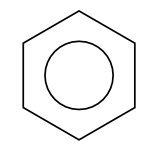
\includegraphics[width=0.4 \textwidth]{../figures/benzene-ring.png}
    \caption{Benzene, \ce{C6H6}, is a colourless, flammable, toxic, and carcinogenic, and has a 
        pleasant odour. It is widely used in the manufacturing of plastics, dyes, synethetic rubber,
        and drugs.}
    \label{fig:benzene-ring}
\end{figure}

\begin{table}[!ht]
    \footnotesize
    \centering
    \caption{Examples of hydrocarbons}
    \setlength{\tabcolsep}{12pt}      % column spacing
    \renewcommand{\arraystretch}{1.2} % row spacing
    \arrayrulecolor{black}            % table border color
    \begin{tabular}{|l|l|l|}
        \hline
        \rowcolor{HeaderColor}
        Hydrocarbon group & Example & Formula \\ \hline
        \multicolumn{3}{|c|}{\textbf{Aliphatic}} \\ \hline
        alkane & ethane & \ce{CH2CH3} \\ \hline
               & cyclohexane & \ce{C6H12} \\ \hline
        alkene & ethene & \ce{CH2CH2} \\ \hline
        alkyne & ethyne & \ce{CHCH} \\ \hline
        \multicolumn{3}{|c|}{\textbf{Aromatic}} \\ \hline
               & benzene & \ce{C6H6} \\ \hline
    \end{tabular}
\end{table}

\lesson{Cyclic Hydrocarbons}
In these compounds, the carbon atoms are connected in such a way to form a ring.
It could be considered that the ends of the carbon chain connect; therefore, there are no terminal 
carbons. As a result, numbering the ring can start at carbon within the ring structure.
\begin{bulleted-list}
    \item To determine whether we use the straight-chain name or the cyclic chain, determine which
        one has more carbons
    \item Cycloalkanes are named by prefixing ``cyclo-''
\end{bulleted-list}

\subsection{Cycloalkenes}
\begin{bulleted-list}
    \item When there is only 1 double bond in the ring and there are no substituent groups, it is not
    necessary to specify the location of the double bond
    \begin{figure}[ht!]
        \centering
        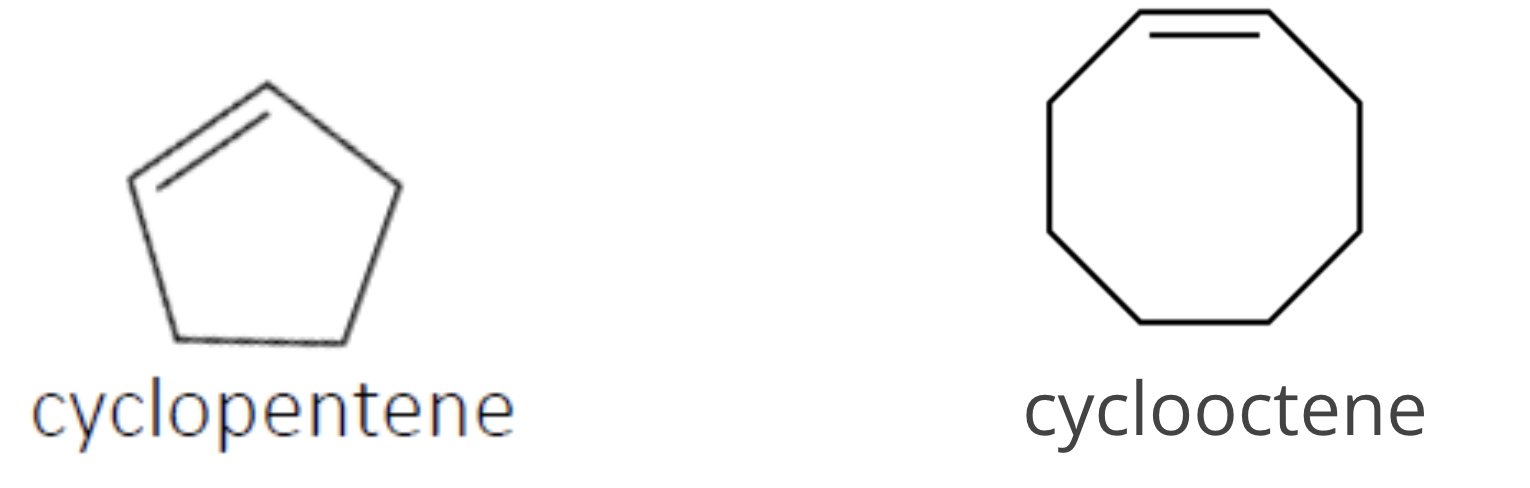
\includegraphics[width=0.6 \textwidth]{../figures/cyclopentene-cyclooctene.png}
    \end{figure}
    \item For substituted cycloalkenes, number the ring in such a way that the carbon atoms of
        the double bond are in the 1- and 2- positions and that also gives the substituents the
        lower number at the first point of difference
        \begin{figure}[ht!]
            \centering
            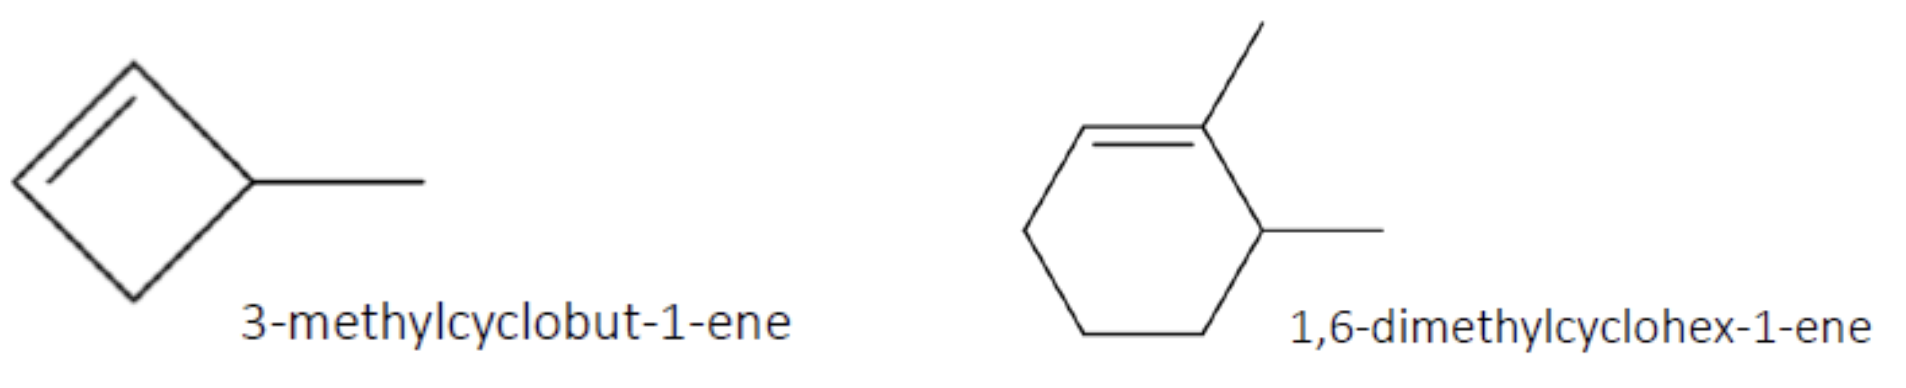
\includegraphics[width=0.6 \textwidth]{../figures/cycloalkenes-substituents.png}
            \caption{When there is a branch, the location of the double bond is also noted
            (always ``-1'')}
        \end{figure}
    \item For cycloalkenes that contain more than one double bond, follow the rules used for alkenes
        \begin{bulleted-list}
            \item Number in the ring in such a way that the carbon atoms of the double bonds result
                in the lowest first point of difference. Location numbers must be provided
            \item If the double bonds don't have a first point of difference, then use the substituent
                groups
            \item If the groups result in the same substituent numbers, order by alphabetical order
        \end{bulleted-list}
        \begin{figure}[ht!]
            \centering
            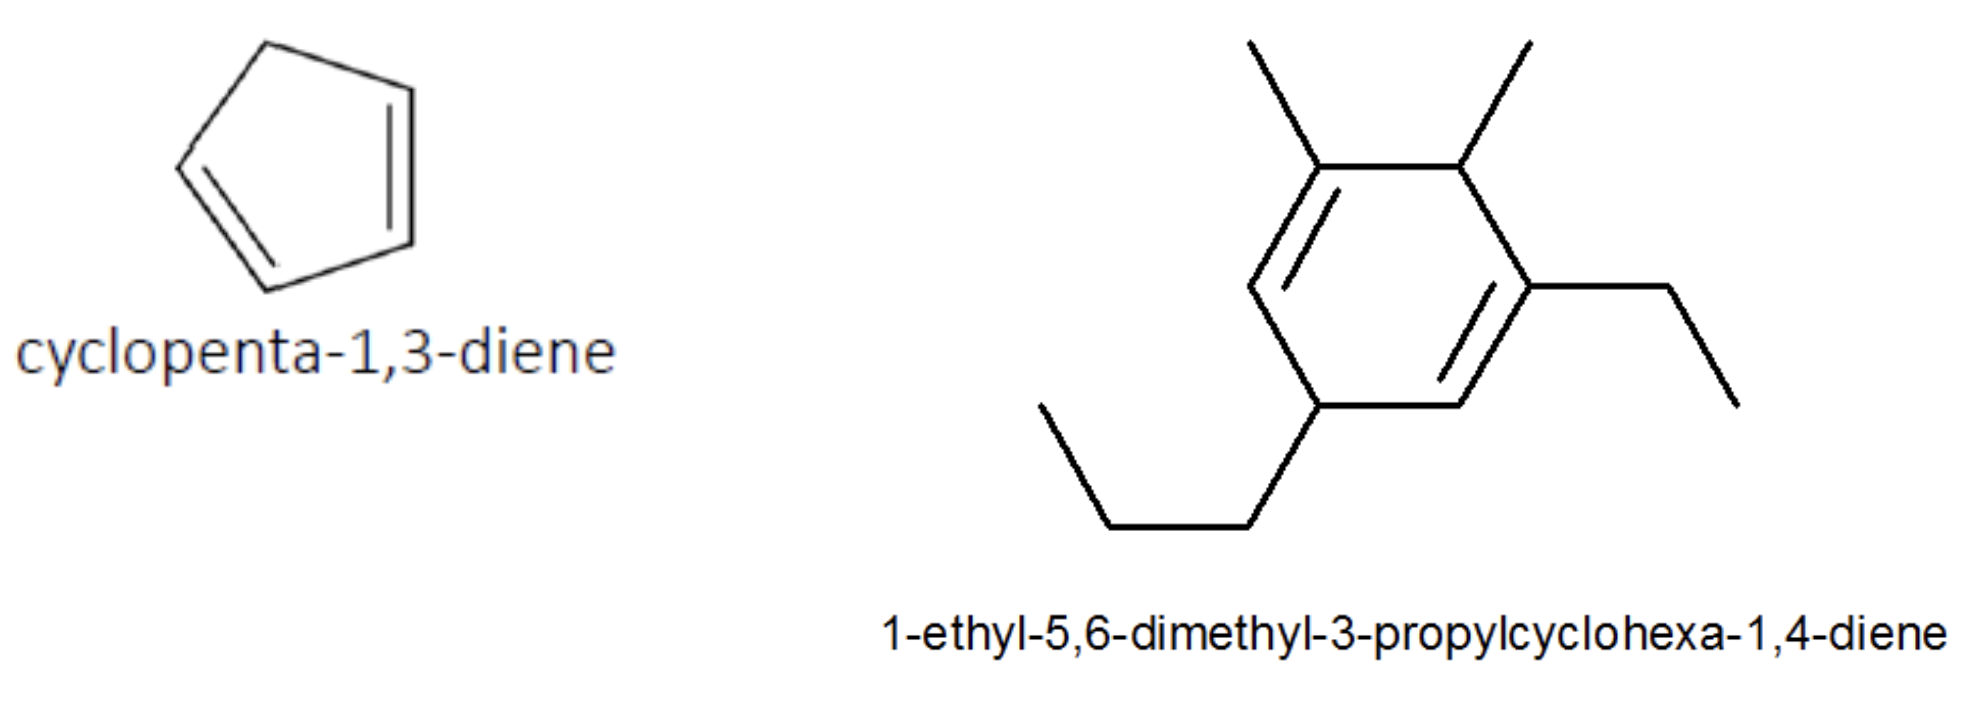
\includegraphics[width=0.6 \textwidth]{../figures/cycloalkenes-examples.png}
        \end{figure}
\end{bulleted-list}
